\documentclass[]{article}
\usepackage{amssymb,amsmath}
\usepackage{hyperref}

\usepackage{todonotes}
\usepackage[margin=2.5cm]{geometry}
\usepackage[super]{natbib}
\bibliographystyle{unsrtnat}

\title{Information Engines: Intelligence and Thermodynamics}
\author{Neil D. Lawrence}
\date{9th January 2021}

\begin{document}


\maketitle


\newcommand{\phaseVariables}{\Gamma}
\newcommand{\stateVariables}{X}
\newcommand{\nullVariables}{{X_0}}
\newcommand{\domainVariables}{{X_1}}
\newcommand{\dataVariables}{Y}
\newcommand{\measuredVariables}{S}
\newcommand{\parameterVector}{W}
\newcommand{\separability}{{F_S}}
\newcommand{\expDist}[2]{\left\langle #1 \right\rangle_{#2}}
\newcommand{\trueProb}{\mathbb{P}}
\newcommand{\simProb}{s}
\newcommand{\domainProb}{\hat{\mathbb{P}}}
\newcommand{\physicsProb}{p}
\newcommand{\approxProb}{q}
\newcommand{\statsProb}{\pi}



\todo{Wonder how this is related to Ashby's concept of "variety",
  e.g. the requisite law of variety:
  \url{https://en.wikipedia.org/wiki/Variety_(cybernetics)}}

\section{Introduction}

This paper attempts to understand the limitations on predictive
modelling by taking a thermodynamic perspective. In particular, is
there a particular definition of intelligence that we can characterise
mathematically and then explore the limits of what might be possible
inspired by physical limitations imposed by the underlying statistical
physics.

Because the paper bridges some different fields, and tries to equate
thermodynamic and information theoretic terms with words that are
widely used in modelling, it may be seen as abusing terminology in
parts. So to clarify at the outset, we are using some general terms in
very specific ways.

In particular, we use the word \emph{simulation} to imply a physical
model over the microstates of the universe that represents our 'best
practical' understanding of the underlying physics. In what follows
this simulation is denoted by
$\physicsProb(\stateVariables|\dataVariables)$. Alongside this we have
the \emph{data model}, which represents the marginal distribution for
the data we observe, $\physicsProb(\dataVariables)$. Quite often in
the below we will refer to this simply as `the model' as it will turn
out to be one of the main objects of focus.

Our investigation is centred around the concept of \emph{free
  energy}. The free energy is the energy in a system that is available
to us for use. In particular we focus on the Helmholtz free energy
which was introduced by Hermann von Helmholtz in the study of
electrochemistry. In a thermodynamic system, the state space is
referred to as the phase space.\footnote{Here we are referring to the
  microstates, the macrostates would be the sufficient statistics of
  the microstates.} The distribution of the phase space is given by
\emph{Boltzmann's distribution} which is derived by considering the
energy levels of different configurations of microstates.  In a
continuous system, we write down the\emph{Hamiltonian} as follows,
\[
\mathbb{P}(\phaseVariables) = \frac{1}{Z_\phaseVariables} \exp(-\beta
E(\phaseVariables)),
\] 
where \(E(\phaseVariables)\) is the energy of the system in microstate
\(\phaseVariables\).

The partition function is then given by 
\[
Z_\phaseVariables = \sum_\phaseVariables \exp(-\beta E(\phaseVariables)),
\] 
where the \(Z\) comes from the German for ``sum over states'' or
\emph{Zustandssumme}, reflecting Boltzmann's Austrian heritage. In the
case of continuous systems we have,
\[
Z_{\phaseVariables} = \frac{1}{h^3}\int \exp(-\beta E(\phaseVariables)) \text{d} \phaseVariables
\] 
and \(E(\phaseVariables)\) is the Hamiltonian of the system.

\subsection{Total Energy}

The total energy, \(U_\phaseVariables\) is defined as the expected
energy,
\[
U_\phaseVariables = \expDist{E(\phaseVariables)}{\trueProb(\phaseVariables)},
\] 
which can be decomposed using the definition of
\(\trueProb(\phaseVariables)\) as 
\[
U_\phaseVariables = A_\phaseVariables + TS_\phaseVariables,
\] 
where 
\[
A_\phaseVariables = - \frac{1}{\beta}\log Z_\phaseVariables
\] 
is the \emph{Helmholtz free energy} and \[ S_\phaseVariables = -k_B
\expDist{\log \trueProb(\phaseVariables)}{\trueProb(\phaseVariables)}
\] is the entropy of the system and \(T\) is the temperature.

This equation expresses a fundamental decomposition of the total
energy into the available energy, \(A_\phaseVariables\) and energy
that is not available, \(TS_\phaseVariables\).

\subsection{Intelligence and Energy} \label{sec-intelligence-and-energy}

We define an intelligent decision to be one that achieves a desired
change of state in our system with the minimum use of resource. In
general, resource would be \emph{time} or \emph{free energy}. For the
moment, time will not enter our calculations because we will focus on
\emph{thermodynamic equilibriums} Which in probability can be thought
of as the \emph{steady state} condition.

Our first step will be to split our phase space into variables we can
observe and the other variables, \(\phaseVariables =
\{\stateVariables, \dataVariables\}\), this allows us to write
\[
U_{\stateVariables,\dataVariables} =
A_{\stateVariables,\dataVariables} +
TS_{\stateVariables,\dataVariables},
\] 
where 
\[
A_{\stateVariables,\dataVariables} = - \frac{1}{\beta}\log
Z_{\stateVariables,\dataVariables}
\] 
and 
\[
S_{\stateVariables,\dataVariables} = -k_B \expDist{\log
  \trueProb({\stateVariables,\dataVariables})}{\trueProb({\stateVariables,\dataVariables})}.
\]
In thermodynamics we might think of the observable values as
'measurable state variables', where as the microstates,
$\stateVariables$, are normally considered to be not directly
measurable. In machine learning though, we might simply think of
$\stateVariables$ as latent variables and $\dataVariables$ as data, or
potential data.

To interact with our system we will introduce a new set of variables,
$\measuredVariables$ which is a $(0,1)$-matrix that contains a one if
a corresponding variable is observed. We place the corresponding
variable in the subscript, so $\measuredVariables_\dataVariables$ is
the matrix that indicates whether or not $\dataVariables$ is
observed. So if we have $\measuredVariables_\dataVariables =
\mathbf{1}$ then all elements of $\dataVariables$ are observed.

We can now denote interactions with the system through changing the
values of $\measuredVariables_\dataVariables$. These interactions will
have their own energy cost that we denote $E(\measuredVariables)$.

If we instantiate the observable states. We change our system. From a
probabilistic perspective, this change is equivalent to
\emph{conditioning} on \(\dataVariables\).

Making an observation in this system is equivalent to conditioning on
\(\dataVariables\) for the total energy which we write as 
\[
U_{\stateVariables|\dataVariables} =
E(\measuredVariables_\dataVariables=\mathbf{1}) +
\expDist{E({\stateVariables|\dataVariables})}{\trueProb({\stateVariables|\dataVariables})},
\]
where we have used $E(\measuredVariables_\dataVariables=\mathbf{1})$
to denote the energy associated with making the observation.

Inspired by probability notation, we decompose that updated energy
state \(E(\stateVariables| \dataVariables)\) into two parts, one which
represents the interaction between our measurements and the state,
\(E(\dataVariables|\stateVariables)\) and \(E(\stateVariables)\)
represents energy terms where there is no interaction and write
\[
\mathbb{P}({\stateVariables|\dataVariables}) =
\frac{1}{Z_{\stateVariables|\dataVariables}} \exp\left(-\beta
E(\dataVariables|\stateVariables) -\beta E(\stateVariables)\right)
\] 
where the partition function is given by
\[
Z_{\stateVariables|\dataVariables} = \int \exp\left(-\beta
E(\dataVariables|\stateVariables) -\beta E(\stateVariables)\right)
\text{d}\stateVariables
\] 
The new total energy, conditioning on the measurements is
\[
U_{\stateVariables|\dataVariables} =
E(\measuredVariables_\dataVariables=\mathbf{1})
A_{\stateVariables|\dataVariables} +
TS_{\stateVariables|\dataVariables}
\] 
where 
\[
A_{\stateVariables|\dataVariables} = - \frac{1}{\beta}\log
Z_{\stateVariables|\dataVariables}
\] 
and 
\[
S_{\stateVariables|\dataVariables} = -k_B \expDist{\log
  \trueProb({\stateVariables|\dataVariables})}{\trueProb({\stateVariables|\dataVariables})}.
\]

We can examine how this changes the free energy, the energy gain
through observation is,
\begin{align*}
  A_{\stateVariables|\dataVariables} -
  A_{\stateVariables,\dataVariables} = & -\frac{1}{\beta} \log
  \frac{Z_{\stateVariables|\dataVariables}}{Z_{\stateVariables,\dataVariables}}\\ &
  -\frac{1}{\beta} \log \trueProb(\dataVariables)
\end{align*}
which is the information gained through the observation,
\(\dataVariables\). This needs to be traded off against the cost of
observing given by $E(\measuredVariables_\dataVariables=\mathbf{1}) $.

This is the fundamental relation between information and energy that
we need to pursue our definition of intelligence. By measuring our
system we gain available energy. If the cost of the measurement is
less than the amount of available energy we gain, then this is an
action worth taking.

\subsection{Intelligence Quotient}

We can define a dimensionless quotient the intelligence of an action
(where action is taken to mean a change of $\measuredVariables$) to
be,
\[
I = \frac{\exp(-\beta E(\measuredVariables_\dataVariables=\mathbf{1}))}{\trueProb(\dataVariables)},\]
where $\beta$ is the thermodynamic temperature \(\beta = \frac{1}{Tk_B}\).

This allows us to express the available energy change as a result of
an action in terms of the intelligence quotient as follows,
\[
\Delta E = T k_B\log I,
\]
so we see that the log intelligence quotient is a critical quantity. 

Since we need to make our decisions about which variables to observe
before we know their values, we can only consider this quotient in
expectation.  and we can also consider the expected available energy
change,
\[
\expDist{\Delta E}{\trueProb(\dataVariables)} = T k_B\expDist{\log I}{\trueProb(\dataVariables)}.
\]
Now we are faced with the problem of approximating the available
energy because we don't have direct access to
$\trueProb(\dataVariables)$.

Our first approach will be to lower bound the expected intelligence
quotient. Introducing a variational distribution
$\simProb(\dataVariables)$, and considering the expected log
intelligence quotient under this distribution we have,
\[
\expDist{\log I}{\simProb(\dataVariables)}   = - \beta E(\measuredVariables_\dataVariables=\textbf{1}) - \expDist{\log \trueProb(\dataVariables)}{\simProb(\dataVariables)}
\]
which is lower bounded by,
\begin{equation}
  \expDist{\log I}{\simProb(\dataVariables)} \geq - \beta
  E(\measuredVariables_\dataVariables=\textbf{1}) - \expDist{\log
    \simProb(\dataVariables)}{\simProb(\dataVariables)}, \label{eqn-lir-lower}
\end{equation}
giving us a lower bound on the expected log intelligence quotient,
where the expectation is taken under the variational
distribution. Maximising this lower bound implies maximising the
entropy of $\simProb(\dataVariables)$. Unfortunately, the entropy is
unbounded. Which implies that the expected intelligence quotient under
a general distribution $\simProb(\dataVariables)$ is also
unbounded. We need more constraints on $\simProb(\cdot)$ to make
progress.

We can rewrite $\log \physicsProb(\dataVariables)$ as
\begin{align}
    \log \trueProb(\dataVariables) & =
    \expDist{\trueProb(\dataVariables,
      \stateVariables)}{\simProb(\stateVariables )} + \expDist{\log
      \simProb(\stateVariables)}{\simProb(\stateVariables)} +
    \text{KL}(\simProb(\stateVariables)||\trueProb(\stateVariables|\dataVariables))
    \nonumber \\ & = -\beta\expDist{ E(\dataVariables |
      \stateVariables)}{\simProb(\stateVariables)}
    -\beta\expDist{E(\stateVariables)}{\simProb(\stateVariables)} -
    \log Z_{\stateVariables,\dataVariables} + \expDist{\log
      \simProb(\stateVariables)}{\simProb(\stateVariables)} +
    \text{KL}(\simProb(\stateVariables)||\trueProb(\stateVariables|\dataVariables)) \label{eqn-true-log-likelihood-1}
\end{align}
and now note that
\[
- \log Z_{\stateVariables,\dataVariables} =
\beta\expDist{E(\dataVariables |
  \stateVariables)}{\simProb(\stateVariables)\trueProb(\dataVariables)}
+ \beta\expDist{E(\stateVariables)}{\simProb(\stateVariables )} -
k_B^{-1}S_\dataVariables -\expDist{\log
  \simProb(\stateVariables)}{\simProb(\stateVariables)} -
\expDist{\text{KL}(\simProb(\stateVariables) ||
  \trueProb(\stateVariables |
  \dataVariables))}{\trueProb(\dataVariables)}
\]
if we now define
\[
\physicsProb(\dataVariables) = \frac{\exp\left(-\beta
  \expDist{E(\dataVariables |
    \stateVariables)}{\simProb(\stateVariables)}\right)}{Z^\prime_\dataVariables}
\]
then we can write
\[
\log \trueProb(\dataVariables) = \log \physicsProb(\dataVariables) +
\text{KL}(\trueProb(\dataVariables)||\physicsProb(\dataVariables)) +
\text{KL}(\simProb(\stateVariables)||\trueProb(\stateVariables|\dataVariables))
-
\expDist{\text{KL}(\simProb(\stateVariables)||\trueProb(\stateVariables|\dataVariables))}{\trueProb(\dataVariables)}.
\]
so we can show that
\[
\log \trueProb(\dataVariables) \geq \log \physicsProb(\dataVariables)
-
\expDist{\text{KL}(\simProb(\stateVariables)||\trueProb(\stateVariables|\dataVariables))}{\trueProb(\dataVariables)}.
\]
Maximizing this lower bound is achieved through minimizing
$\expDist{\text{KL}(\simProb(\stateVariables)||\trueProb(\stateVariables|\dataVariables))}{\trueProb(\dataVariables)}$,
in other words, finding a variational distribution which represents
how the microstates behave correctly. Maximising this bound improves
the physical plausibility of the model. We call
$\simProb(\stateVariables)$ the \emph{simulation} and we call
$\exp\left(-
\expDist{\text{KL}(\simProb(\stateVariables)||\trueProb(\stateVariables|\dataVariables))}{\trueProb(\dataVariables)}\right)$
the global simulation fidelity, $F_G$,
\[
\log F_G =
-\expDist{\text{KL}(\simProb(\stateVariables)||\trueProb(\stateVariables|\dataVariables))}{\trueProb(\dataVariables)}.
\]
Note that the fidelities we define vary between 0 and 1, with 1 being
equivalent to 100\% faithful, meaning that the match between the two
distributions is perfect.

This in turn gives us an upper bound on our log intelligence quotient,
\[
\log I \leq -\beta E(\measuredVariables_\dataVariables = \textbf{1})
-\log \physicsProb(\dataVariables) - \log F_G.
\]
So we can write the intelligence quotient as,
\[
I \leq
\frac{1}{F_G}\frac{\exp\left(-E(\measuredVariables_\dataVariables=\textbf{1})\right)}{\physicsProb(\dataVariables)}.
\]

\subsection{Lower Bound}

We can also write
\[
- \log Z_{\stateVariables,\dataVariables} =
\beta\expDist{E(\dataVariables |
  \stateVariables)}{\simProb(\stateVariables)\physicsProb(\dataVariables)}
+ \beta\expDist{E(\stateVariables)}{\simProb(\stateVariables )} +
\expDist{\log \trueProb(\dataVariables)}{\physicsProb(\dataVariables)}
-\expDist{\log \simProb(\stateVariables)}{\simProb(\stateVariables)} -
\expDist{\text{KL}(\simProb(\stateVariables) ||
  \physicsProb(\stateVariables |
  \dataVariables))}{\physicsProb(\dataVariables)}
\]
which substituting into (\ref{eqn-true-log-likelihood-1}) gives
\[
\log \trueProb(\dataVariables) = \log \physicsProb(\dataVariables) +
\text{KL}(\simProb(\stateVariables)||\trueProb(\stateVariables|\dataVariables))
- \text{KL}(\physicsProb(\dataVariables) || \trueProb(\dataVariables))
- \expDist{\text{KL}(\simProb(\stateVariables) ||
  \physicsProb(\stateVariables |
  \dataVariables))}{\physicsProb(\dataVariables)}
\]
and a corresponding \emph{upper} bound on $\log \trueProb(\dataVariables)$, 
\[
\log \trueProb(\dataVariables) \leq \log \physicsProb(\dataVariables)
+
\text{KL}(\simProb(\stateVariables)||\trueProb(\stateVariables|\dataVariables)).
\]
We define the $\exp\left(-
\text{KL}(\simProb(\stateVariables)||\trueProb(\stateVariables|\dataVariables))\right)$
to be the \emph{contextual} simulation fidelity, $F_C$,
\[
\log F_C =
-\text{KL}(\simProb(\stateVariables)||\trueProb(\stateVariables|\dataVariables)).
\]
and note the relationship between the contextual and global simulation
fidelities,
\[
\log F_G = \expDist{\log F_C}{\trueProb(\dataVariables)}.
\]
and we can now lower bound the intelligence quotient,
\[
I \geq F_C \frac{\exp\left(-E(\measuredVariables_\dataVariables=
  \textbf{1})\right)}{\physicsProb(\dataVariables)}.
\]
giving us a range for the intelligence quotient,
\[
F_C \frac{\exp\left(-E(\measuredVariables_\dataVariables=
  \textbf{1})\right)}{\physicsProb(\dataVariables)} \leq I \leq
\frac{1}{F_G}\frac{\exp\left(-E(\measuredVariables_\dataVariables=
  \textbf{1})\right)}{\physicsProb(\dataVariables)}.
\]

\subsection{Global and Local Simulations}

The two different simulation fidelities represent a fundamental
tension in modelling. The global simulation fidelity gives us a
simulation that tries to be valid across the different data that we
might observe, $\trueProb(\dataVariables)$. The local simulation
fidelity is specific to the data we have, $\dataVariables$. The global
simulation fidelity is associated with our global understanding of
physical laws. The contextual simulation fidelity is associated with
the particular circumstance we currently find ourselves in.



\begin{figure}
    \centering
    \def\svgwidth{\textwidth}
   %% Creator: Inkscape 1.0.2 (e86c8708, 2021-01-15), www.inkscape.org
%% PDF/EPS/PS + LaTeX output extension by Johan Engelen, 2010
%% Accompanies image file 'py-bounds.pdf' (pdf, eps, ps)
%%
%% To include the image in your LaTeX document, write
%%   \input{<filename>.pdf_tex}
%%  instead of
%%   \includegraphics{<filename>.pdf}
%% To scale the image, write
%%   \def\svgwidth{<desired width>}
%%   \input{<filename>.pdf_tex}
%%  instead of
%%   \includegraphics[width=<desired width>]{<filename>.pdf}
%%
%% Images with a different path to the parent latex file can
%% be accessed with the `import' package (which may need to be
%% installed) using
%%   \usepackage{import}
%% in the preamble, and then including the image with
%%   \import{<path to file>}{<filename>.pdf_tex}
%% Alternatively, one can specify
%%   \graphicspath{{<path to file>/}}
%% 
%% For more information, please see info/svg-inkscape on CTAN:
%%   http://tug.ctan.org/tex-archive/info/svg-inkscape
%%
\begingroup%
  \makeatletter%
  \providecommand\color[2][]{%
    \errmessage{(Inkscape) Color is used for the text in Inkscape, but the package 'color.sty' is not loaded}%
    \renewcommand\color[2][]{}%
  }%
  \providecommand\transparent[1]{%
    \errmessage{(Inkscape) Transparency is used (non-zero) for the text in Inkscape, but the package 'transparent.sty' is not loaded}%
    \renewcommand\transparent[1]{}%
  }%
  \providecommand\rotatebox[2]{#2}%
  \newcommand*\fsize{\dimexpr\f@size pt\relax}%
  \newcommand*\lineheight[1]{\fontsize{\fsize}{#1\fsize}\selectfont}%
  \ifx\svgwidth\undefined%
    \setlength{\unitlength}{841.88976378bp}%
    \ifx\svgscale\undefined%
      \relax%
    \else%
      \setlength{\unitlength}{\unitlength * \real{\svgscale}}%
    \fi%
  \else%
    \setlength{\unitlength}{\svgwidth}%
  \fi%
  \global\let\svgwidth\undefined%
  \global\let\svgscale\undefined%
  \makeatother%
  \begin{picture}(1,0.70707071)%
    \lineheight{1}%
    \setlength\tabcolsep{0pt}%
    \put(0,0){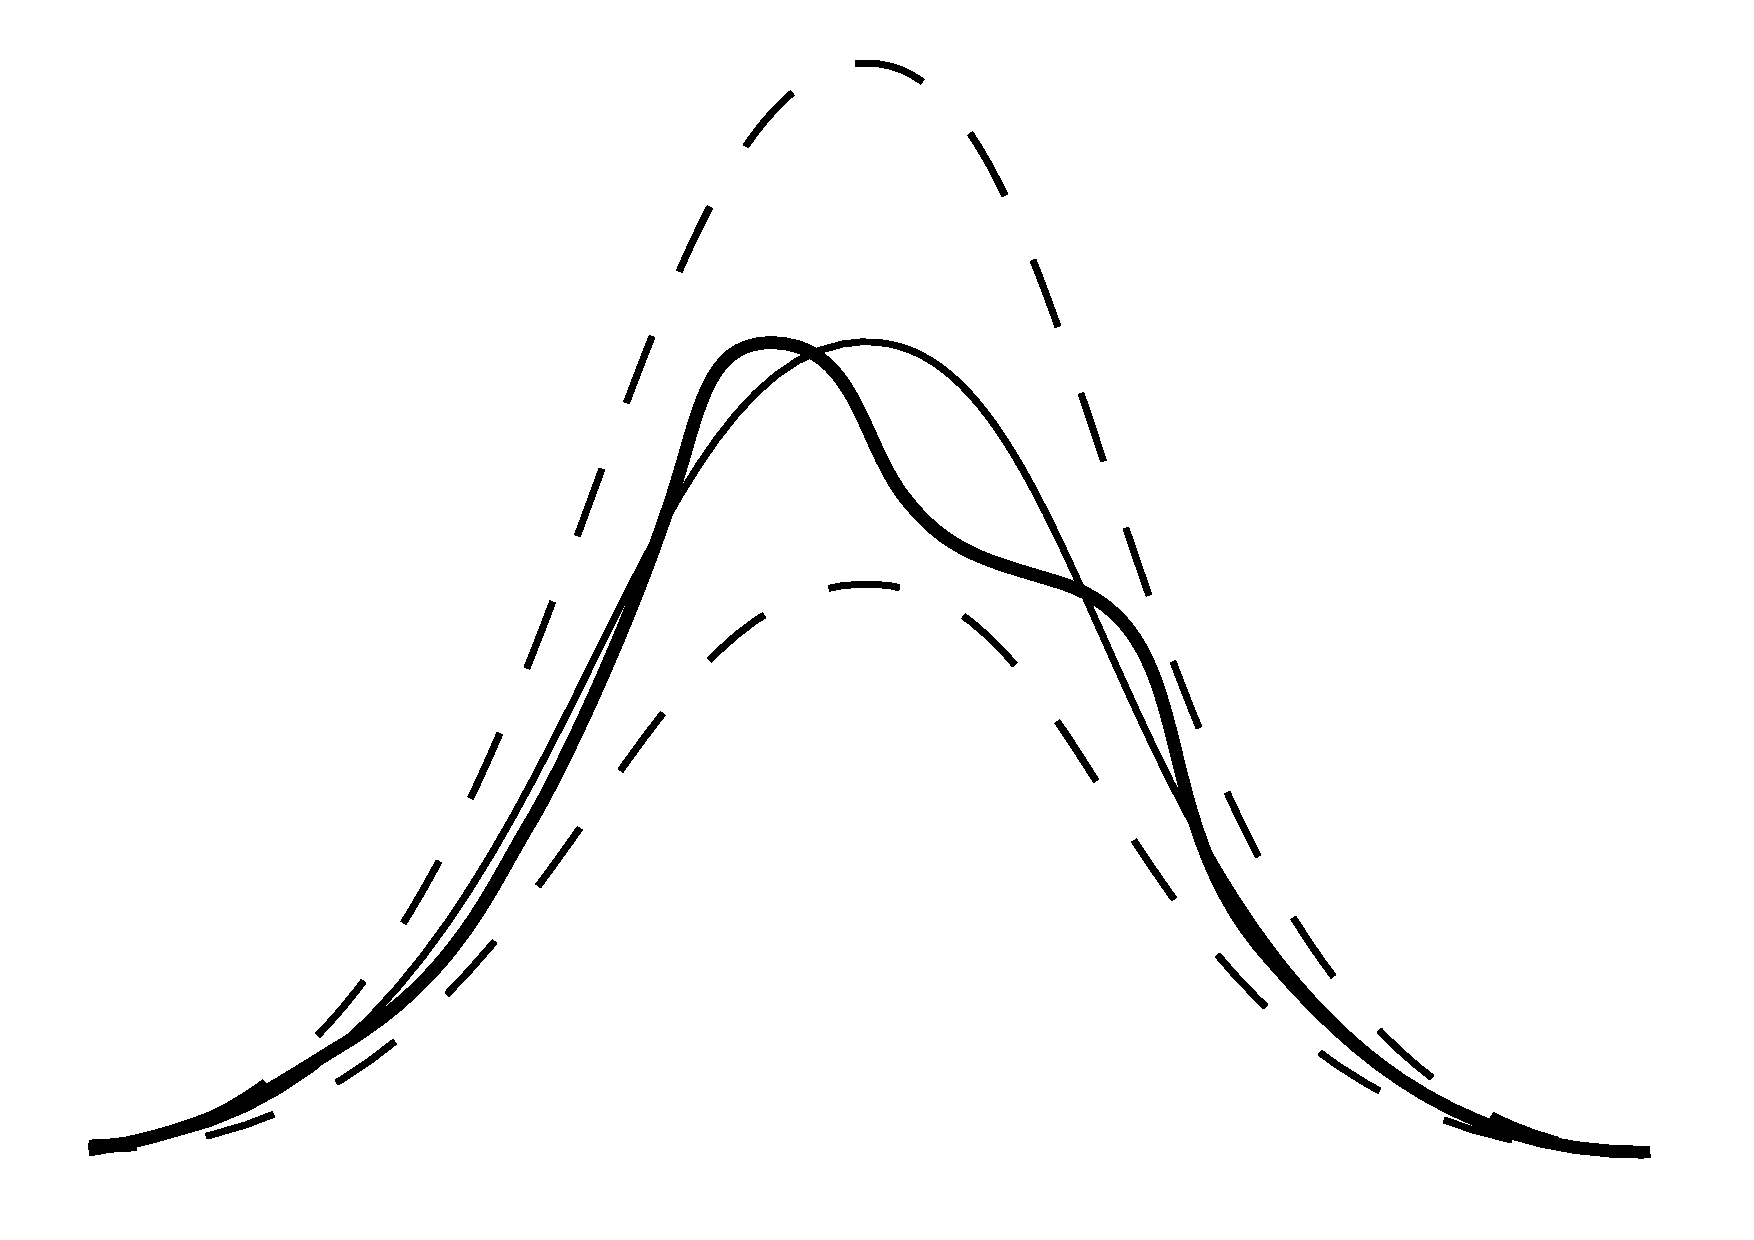
\includegraphics[width=\unitlength,page=1]{py-bounds.pdf}}%
    \put(0.39432495,0.40447998){$\trueProb(Y)$}%
    \put(0.40333575,0.27675171){$F_C \physicsProb(Y)$}%
    \put(0.67081228,0.6197671){$\frac{1}{F_G}\physicsProb(Y)$}%
    \put(0.48646448,0.53538479){$p(Y)$}%
  \end{picture}%
\endgroup%

    \caption{Visualisation of the lower and upper bound on
      $\trueProb(\dataVariables)$ to highlight how the approximation,
      $\physicsProb(\dataVariables)$, corresponds to the bounds
      combining with the fidelities, $F_C$.}
    \label{fig-py-bounds}
\end{figure}



\begin{figure}
  \centering
  \def\svgwidth{\textwidth}
    %% Creator: Inkscape 1.0.2 (e86c8708, 2021-01-15), www.inkscape.org
%% PDF/EPS/PS + LaTeX output extension by Johan Engelen, 2010
%% Accompanies image file 'log-py-bounds.pdf' (pdf, eps, ps)
%%
%% To include the image in your LaTeX document, write
%%   \input{<filename>.pdf_tex}
%%  instead of
%%   \includegraphics{<filename>.pdf}
%% To scale the image, write
%%   \def\svgwidth{<desired width>}
%%   \input{<filename>.pdf_tex}
%%  instead of
%%   \includegraphics[width=<desired width>]{<filename>.pdf}
%%
%% Images with a different path to the parent latex file can
%% be accessed with the `import' package (which may need to be
%% installed) using
%%   \usepackage{import}
%% in the preamble, and then including the image with
%%   \import{<path to file>}{<filename>.pdf_tex}
%% Alternatively, one can specify
%%   \graphicspath{{<path to file>/}}
%% 
%% For more information, please see info/svg-inkscape on CTAN:
%%   http://tug.ctan.org/tex-archive/info/svg-inkscape
%%
\begingroup%
  \makeatletter%
  \providecommand\color[2][]{%
    \errmessage{(Inkscape) Color is used for the text in Inkscape, but the package 'color.sty' is not loaded}%
    \renewcommand\color[2][]{}%
  }%
  \providecommand\transparent[1]{%
    \errmessage{(Inkscape) Transparency is used (non-zero) for the text in Inkscape, but the package 'transparent.sty' is not loaded}%
    \renewcommand\transparent[1]{}%
  }%
  \providecommand\rotatebox[2]{#2}%
  \newcommand*\fsize{\dimexpr\f@size pt\relax}%
  \newcommand*\lineheight[1]{\fontsize{\fsize}{#1\fsize}\selectfont}%
  \ifx\svgwidth\undefined%
    \setlength{\unitlength}{841.88976378bp}%
    \ifx\svgscale\undefined%
      \relax%
    \else%
      \setlength{\unitlength}{\unitlength * \real{\svgscale}}%
    \fi%
  \else%
    \setlength{\unitlength}{\svgwidth}%
  \fi%
  \global\let\svgwidth\undefined%
  \global\let\svgscale\undefined%
  \makeatother%
  \begin{picture}(1,0.70707071)%
    \lineheight{1}%
    \setlength\tabcolsep{0pt}%
    \put(0,0){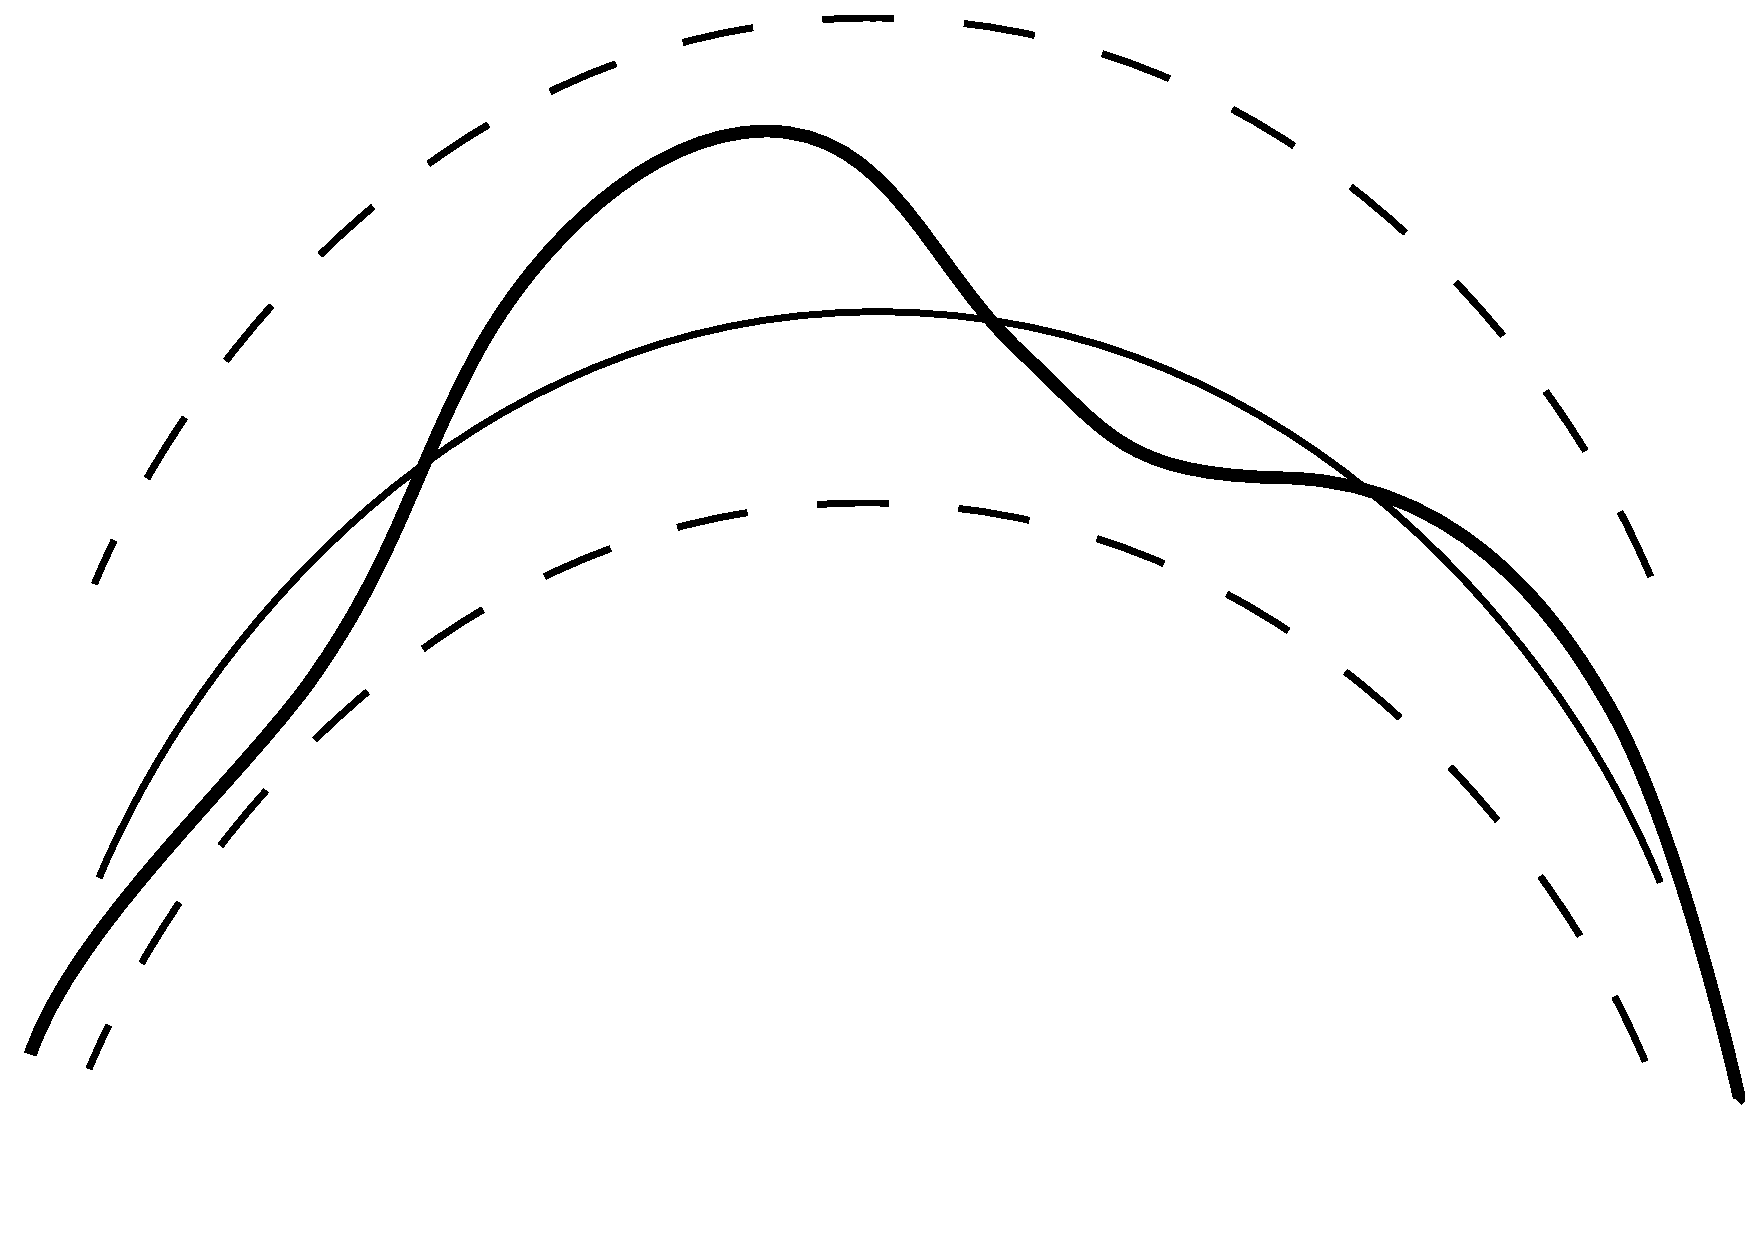
\includegraphics[width=\unitlength,page=1]{./diagrams/log-py-bounds.pdf}}%
    \put(0.55054713,0.58056959){\Large $\log \trueProb(\dataVariables)$}%
    \put(0.31892536,0.34449357){\Large $\log \physicsProb(\dataVariables) + \log F_C$}%
    \put(0.67081228,0.66609147){\Large $\log \physicsProb(\dataVariables) - \log F_G$}%
    \put(0.39197527,0.46832211){\Large $\log \physicsProb(\dataVariables)$}%
  \end{picture}%
\endgroup%

    \caption{Visualisation of the lower and upper bound on $\log
      \trueProb(\dataVariables)$ to highlight how the approximation,
      $\log \physicsProb(\dataVariables)$, corresponds to the bounds
      combining with the fidelities, $\log F_C$ and $\log F_G$.}
    \label{fig-log-py-bounds}
\end{figure}


\section{Maximizing Intelligence Quotient}

The intelligence quotient can be maximized by maximizing the lower bound with respect to $\simProb(\stateVariables)$, which in turn gives us the optimal form of $\physicsProb(\dataVariables)$. The lower bound on the log intelligence quotient is given by,
\[
\log I \geq - \log \physicsProb(\dataVariables) -\text{KL}(\simProb(\stateVariables)||\trueProb(\stateVariables|\dataVariables)) - \beta E(\measuredVariables_\dataVariables = \textbf{1})
\]
recalling that $\log \physicsProb = \frac{\expDist{E(\dataVariables|\stateVariables)}{\simProb(\stateVariables)}}{Z^\prime_\dataVariables}$ and focussing on the terms that are dependent on $\simProb(\stateVariables)$ we have,
\[
\log I \geq \beta \expDist{E(\stateVariables)}{\simProb(\stateVariables)} - \expDist{\log \simProb(\stateVariables)}{\simProb(\stateVariables)} + \text{const.},
\]
where $\text{const.} = \log Z^\prime_Y - \log Z_{\stateVariables|\measuredVariables}$. This can be maximized by setting,
\[
\simProb(\stateVariables) = \trueProb(\stateVariables)
\]
giving us the unsurprising conclusion that the maximum intelligence quotient is given by setting our simulation to be equal to the true distribution of the microstates, $\trueProb(\stateVariables)$. 

However, this is generally impractical. In our set up $\stateVariables$, includes all the microstates of the Universe. We are unlikely to be able to build an accurate simulation across all these variables. So our first step is to constrain our simulation such that it focuses on variables of interest.

\subsection{Null Space and Domain Space}

We divide the microstates of the Universe into two parts, we call one the null space, and denote it by $\nullVariables$. These are the microstates in the Universe that we'd prefer to ignore in our simulation. Then we have the domain space, which we denote by $\domainVariables$. These are the microstates that we considere directly relevant for our problem. So that we can factorise our Universe into different simulations for use in different contexts, we then make the assumption that
\[
\simProb(\stateVariables) = \simProb(\nullVariables) \simProb(\domainVariables)
\]
and we impose this as a constraint when maximizing the lower bound on the intelligence quotient.

Under this constraint, we obtain the following form for $\simProb(\domainVariables)$,
\[
\simProb(\domainVariables) = \frac{\exp \left(-\beta E^\prime(\domainVariables)\right)}{Z^\prime_\domainVariables},
\]
where we have introduced $E^\prime(\domainVariables) = \expDist{E(\stateVariables)}{\simProb(\nullVariables)}$ as well as the domain simulation's partition function, $Z^\prime_\domainVariables$.

Note that there is now an interdependence between the optimal form for $\simProb(\domainVariables)$ and $\simProb(\nullVariables)$

We can write the lower bound as,
$$
\log I \geq -\log \physicsProb(\dataVariables) - \expDist{\text{KL}\left(\simProb(\domainVariables) || \frac{\trueProb(\dataVariables | \domainVariables,\nullVariables)\simProb(\domainVariables)}{\trueProb(\dataVariables)}\right)}{\simProb(\nullVariables)}  - \expDist{\log \frac{\simProb(\domainVariables)\simProb(\nullVariables)}{\trueProb(\domainVariables,\nullVariables)}}{\simProb(\domainVariables)\simProb(\nullVariables)}  -\beta E(\measuredVariables_\dataVariables=\textbf{1})
$$
$$
\log I \geq -\log \physicsProb(\dataVariables) + \log F_\domainVariables  + \log \separability  -\beta E(\measuredVariables_\dataVariables=\textbf{1})
$$
where we have introduced the \emph{separability}, $\separability$,
$$
\log \separability = - \text{KL}\left(\simProb(\domainVariables)\simProb(\nullVariables)||\trueProb(\domainVariables,\nullVariables)\right)
$$
which represents how separable our choice of domain space and null space are in reality,
and also we have defined,
$$
\log F_\domainVariables = - \expDist{\text{KL}\left(\simProb(\domainVariables) || \frac{\trueProb(\dataVariables | \domainVariables,\nullVariables)\simProb(\domainVariables)}{\trueProb(\dataVariables)}\right)}{\simProb(\nullVariables)},
$$
as the domain fidelity. If the domain variables are selected such that,
$$
\trueProb(\dataVariables | \domainVariables, \nullVariables) = \trueProb(\dataVariables |\domainVariables)
$$
then we can write
$$
\log F_\domainVariables = - \text{KL}\left(\simProb(\domainVariables) || \domainProb(\domainVariables | \dataVariables) \right),
$$
where
$$
\domainProb(\domainVariables | \dataVariables) = \frac{\trueProb(\dataVariables | \domainVariables)\simProb(\domainVariables)}{\trueProb(\dataVariables)}
$$

\section{Parameters}

We now introduce a set of auxiliary variables, $\parameterVector$. These auxiliary variables augment the domain distribution,
\[
\domainProb(\domainVariables | \dataVariables) = \int \domainProb(\domainVariables, \parameterVector | \dataVariables) \text{d} \parameterVector,
\]
allowing us to lower bound the logarithm of the domain probability,
\[
\log \domainProb(\domainVariables | \dataVariables) \geq \int \simProb(\parameterVector|\domainVariables) \log \frac{\domainProb(\domainVariables, \parameterVector | \dataVariables)}{\simProb(\parameterVector|\domainVariables)} \text{d}\parameterVector,
\]
which in turn allows us to lower bound the domain fidelity, 
\[
\log F_\domainVariables = \int \simProb(\domainVariables) \log \frac{\domainProb(\domainVariables | \dataVariables)}{\simProb(\domainVariables)} \geq \int \simProb(\parameterVector,\domainVariables) \log \frac{\domainProb(\domainVariables, \parameterVector | \dataVariables)}{\simProb(\parameterVector,\domainVariables)} \text{d}\parameterVector,
\]
which we can rewrite as
\[
\log F_\domainVariables \geq \int \simProb(\parameterVector) \log \frac{\domainProb(\parameterVector|\dataVariables)}{\simProb(\parameterVector)}\text{d} \parameterVector + \int \simProb(\parameterVector) \int \simProb(\domainVariables|\parameterVector) \log \frac{\domainProb(\domainVariables|\parameterVector, \dataVariables)}{\simProb(\domainVariables|\parameterVector)} \text{d} \domainVariables \text{d}\parameterVector,
\]
or in terms of KL divergences,
\begin{align*}
\log F_\domainVariables \geq & -\text{KL}\left(\simProb(\parameterVector)|| \domainProb(\parameterVector|\dataVariables)\right) - \expDist{ \text{KL}\left(\simProb(\domainVariables|\parameterVector) || \domainProb(\domainVariables|\parameterVector, \dataVariables) \right)}{ \simProb(\parameterVector)} \\
\log F_\domainVariables \geq & \log F_\parameterVector + \log R_{\domainVariables|\parameterVector}
\end{align*}
which in turn implies that
$$
F_\domainVariables \geq F_\parameterVector R_{\domainVariables|\parameterVector}
$$
where $F_\parameterVector$ is the parameter fidelity and $R_{\domainVariables|\parameterVector}$ is the representability. 

Parameterizing the model has allowed us to decompose the domain fidelity into a parameter fidelity and a representability. To see why we call $F_{\domainVariables |\parameterVector}$ the representability, we first minimizing the lower bound on the intelligence quotient with respect to $\simProb(\domainVariables | \parameterVector)$ and we recover,
$$
\simProb(\domainVariables | \parameterVector) = \domainProb(\domainVariables | \parameterVector).
$$
In which case the representability is given by, 
$$
\log R_{\domainVariables | \parameterVector} = \expDist{ \text{KL}\left(\domainProb(\domainVariables|\parameterVector) || \domainProb(\domainVariables|\parameterVector, \dataVariables) \right)}{ \simProb(\parameterVector)}.
$$
This KL divergence will be zero (and the representability 1) only if conditioning on $\dataVector$ does not change the domainprobability. In other words if $\parameterVector$ renders the domain variables conditionally independent of the data. In other words, storing the parameters is sufficient for us to have all the information about the domain variables, we don't need to store the data itself. For this to happen $\parameterVector$ would have to be sufficiently large to represent all the information in $\dataVector$.
\todo{I think this is all true. Firstly, the minima of the bound (but it relies on $E(Y|X)$ in $p(Y)$ matching that in $\domainProb()$. And secondly that this implies conditional independence if W is large enough ... might need some conditions on a DAG between W, X1 and Y.} 

Minimizing the lower bound on the intelligence quotient with respect to $\simProb(\parameterVector)$ recovers,
$$
\simProb(\parameterVector) = \domainProb(\parameterVector)
$$
\todo{Need to prove these two statements, I think they work if the $E(Y|X)$ term inside the P from the KL divergence matches the $E(Y|X)$ inside the $p(Y)$} 

\section{Model Selection}

In practice, we want to find the tightest bound on the intelligence ratio. Above we've shown what the form 


Some thoughts:

\begin{enumerate}
    \item Choose parameters such that $\physicsProb(\dataVariables|\parameterVector) = \prod_{i=1}^n \physicsProb(\dataPoint_i |\parameterVector)$
    \item Choosing robust models ... what about heavy tailed vs light tailed $\physicsProb(\dataPoint_i |\parameterVector)$. 
\end{enumerate}

Also for a fixed data set $\dataVariables$, the actual intelligence quotient is fixed. And we are supposed to be computing a lower bound. 

Imagine we have two models, and one model has a higher negative log probability than the other. It doesn't mean it's got a higher intelligence quotient, because that's fixed. Instead, it means our estimate of the intelligence coefficient is likely to be over optimistic. 

It feels likely there's some minimax stuff going on here. We want the model $\physicsProb(\dataVariables)$ which minimise the maximum ... because this will be the one with the highest fidelity and representability. Need to formalise that argument.

\end{document}
